\documentclass[a4j]{jarticle} %jsrticleでもいい
\usepackage{fancyhdr} %ヘッダーを表示させるのに必要
%\usepackage{listings, jlisting} %ソースコードを貼り付けるのに必要
\usepackage{listings} %ソースコードを貼り付けるのに必要
\usepackage{color}
\usepackage{comment} %複数行のコメントアウトのパッケージ
\usepackage{amsmath,amssymb}
\usepackage[dvipdfmx]{graphicx}
\usepackage{here}
\usepackage{ascmac}
\setlength{\parindent}{0pt}
\lstset{
  basicstyle={\ttfamily},
  backgroundcolor={\color[gray]{.90}},
  identifierstyle={\small},
  commentstyle={\smallitshape},
  keywordstyle={\small\bfseries},
  ndkeywordstyle={\small},
  stringstyle={\small\ttfamily},
  frame={tb},
  breaklines=true,
  columns=[l]{fullflexible},
  %numbers=left, %行番号を表示する
  xrightmargin=1zw,
  xleftmargin=2zw,
  numberstyle={\scriptsize},
  stepnumber=1,
  numbersep=1zw,
  lineskip=-0.5ex
}

\pagestyle{fancy}
  \lhead{メディア情報学プログラミング演習} %ヘッダー左
  \rhead{J1-26} %ヘッダー右
\topmargin =-15mm %ページ上部の隙間の調整

\title{令和6年度 メディア情報学プログラミング演習\\グループプログラミング レポート\\料理提供ゲーム「MiniCook」}
\renewcommand{\lstlistingname}{コード}
\begin{document}
\maketitle

\begin{center}%中央に表書く
  \begin{tabular}{|c||c|}
      \hline
      学科&情報理工学域\\
      \hline
      クラス&J1\\
      \hline
      グループ番号&26\\
      \hline
      2210259&米谷祐希\\
      \hline
      2210730&鈴木早紀\\
      \hline
      2210743&吉田陽音\\
      \hline
  \end{tabular}
\end{center}

\newpage

\section{概要説明}
 このゲームは、レストランで働くプレイヤーが、制限時間内に料理を作るゲームである。以下の料理提供までの手順を繰り返すことでポイントを獲得し、制限時間終了時にスコアとレベルが表示される。
\begin{enumerate}
  \item オーダーの確認\par
   まず、画面上部にランダムにオーダーが提示される。オーダーには、使う食材と調理方法が記載されている。各オーダーにはそれぞれ制限時間が設定されており、残り時間はオーダー上のゲージにリアルタイムに表示される。
  \item 食材の調理\par
   次に、オーダーに記載されている食材を、各食材ボックスから取り出す。各食材を持ったまま、各調理器具の前でアクションボタンを押すことで、食材が加工される。
  \item 料理の完成と提供\par
   料理は、加工された食材とお皿を組み合わせることで完成する。それらを組み合わせて料理ができあがれば、提供口に置くことで提供となり、オーダーと一致しているか判定される。一致していれば加点、間違っていれば減点となる。   
\end{enumerate}
 また、ゲームは3画面に分かれており、スタート画面、ゲーム画面、リザルト画面がある。また、各画面や各動作にはBGMや効果音がついている。操作はキーボードのA,S,D,W,J,K,Spaceキーを用いている。\par
 作業はGitHubを用い保存・共有を行った。米谷がModelと全体の管理、鈴木がView、吉田がControllerを主に担当したが、最終的には各自の担当領域を超えて協力しながら取り組んだ。


\section{設計方針}
 MVCモデルを用い設計した。図1にクラス図を示す。
\begin{figure}[H]
  \begin{center}
  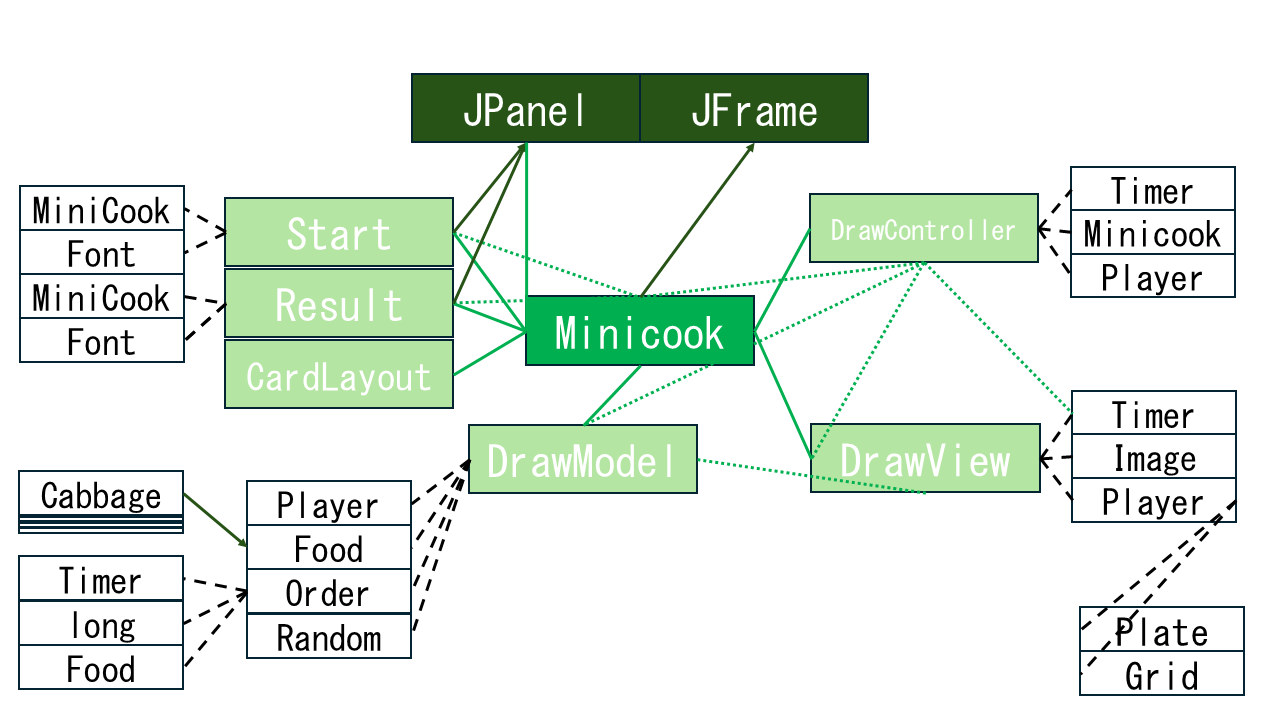
\includegraphics[scale=0.3]{img/class.png}
  \caption{クラス図}
  \end{center}
\end{figure}



\section{プログラムの説明}


\section{実行例}


\section{考察}


\section{感想}
\subsection*{(米谷祐希)}

\subsection*{(鈴木早紀)}

\subsection*{(吉田陽音)}



\newpage
\section*{付録1:操作マニュアル}



\newpage
\section*{付録2:プログラムリスト}



\end{document}

\begin{comment}
\end{comment}